%
% folgerungen.tex
%
% (c) 2021 Prof Dr Andreas Müller, OST Ostschweizer Fachhochschule
%
\bgroup
\def\sx{1}
\definecolor{darkgreen}{rgb}{0,0.6,0}
\begin{frame}[t]
\frametitle{Folgerungen}
\vspace{-10pt}
\begin{columns}[t]
\begin{column}{0.30\textwidth}
\begin{block}{Zunahme}
Für alle $k<l$ gilt
\begin{align*}
\mathcal{J}^k(f) &\supsetneq \mathcal{J}^{k+1}(f)
\\
\mathcal{K}^k(f) &\subsetneq \mathcal{K}^{k+1}(f)
\end{align*}
Für $k\ge l$ gilt
\begin{align*}
\mathcal{J}^k(f) &= \mathcal{J}^{k+1}(f)
\\
\mathcal{K}^k(f) &= \mathcal{K}^{k+1}(f)
\end{align*}
Ausserdem ist $l\le n$
\end{block}
\end{column}
\begin{column}{0.66\textwidth}
\begin{center}
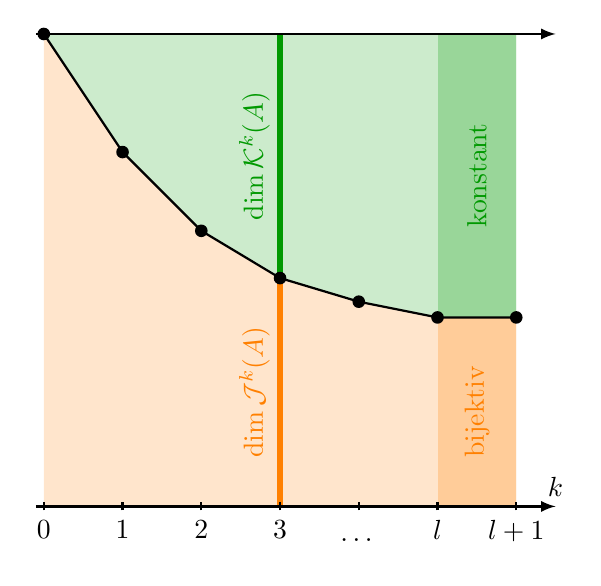
\begin{tikzpicture}[>=latex,thick]
\def\pfad{
	({0*\sx},6) --
	({1*\sx},4.5) --
	({2*\sx},3.5) --
	({3*\sx},2.9) --
	({4*\sx},2.6) --
	({5*\sx},2.4) --
	({6*\sx},2.4)
}

\fill[color=orange!20] \pfad -- ({6*\sx},0) -- (0,0) -- cycle;
\fill[color=darkgreen!20] \pfad -- ({6*\sx},6) -- cycle;
\fill[color=orange!40] ({5*\sx},0) rectangle ({6*\sx},2.4);
\fill[color=darkgreen!40] ({5*\sx},6) rectangle ({6*\sx},2.4);

\draw[color=darkgreen,line width=2pt] ({3*\sx},6) -- ({3*\sx},2.9);
\node[color=darkgreen] at ({3*\sx},4.45) [rotate=90,above] {$\dim\mathcal{K}^k(A)$};
\draw[color=orange,line width=2pt] ({3*\sx},0) -- ({3*\sx},2.9);
\node[color=orange] at ({3*\sx},1.45) [rotate=90,above] {$\dim\mathcal{J}^k(A)$};

\node[color=orange] at ({5.5*\sx},1.2) [rotate=90] {bijektiv};
\node[color=darkgreen] at ({5.5*\sx},4.2) [rotate=90] {konstant};

\fill ({0*\sx},6) circle[radius=0.08];
\fill ({1*\sx},4.5) circle[radius=0.08];
\fill ({2*\sx},3.5) circle[radius=0.08];
\fill ({3*\sx},2.9) circle[radius=0.08];
\fill ({4*\sx},2.6) circle[radius=0.08];
\fill ({5*\sx},2.4) circle[radius=0.08];
\fill ({6*\sx},2.4) circle[radius=0.08];

\draw \pfad;

\draw[->] (-0.1,0) -- ({6*\sx+0.5},0) coordinate[label={$k$}];
\draw[->] (-0.1,6) -- ({6*\sx+0.5},6);

\foreach \x in {0,...,6}{
	\draw (\x,-0.05) -- (\x,0.05);
}
\foreach \x in {0,...,3}{
	\node at ({\x*\sx},-0.05) [below] {$\x$};
}
\node at ({4*\sx},-0.05) [below] {$\dots\mathstrut$};
\node at ({5*\sx},-0.05) [below] {$l$};
\node at ({6*\sx},-0.05) [below] {$l+1$};

\end{tikzpicture}
\end{center}
\end{column}
\end{columns}
\end{frame}
\egroup
